\documentclass{article}

\usepackage[utf8x]{inputenc}
\usepackage[english,russian]{babel}
\usepackage{amsmath,amscd}
\usepackage{amsthm}
\usepackage{amsfonts}
\usepackage{amssymb}
\usepackage{cmap}
\usepackage{centernot}
\usepackage{enumitem}
\usepackage{perpage}
\usepackage{chngcntr}
\usepackage{graphicx}
\usepackage[bookmarks=true,pdfborder={0 0 0 }]{hyperref}
\usepackage{indentfirst}
\usepackage{tikz}
\usetikzlibrary{arrows,automata,positioning}
\hypersetup{
  colorlinks,
  citecolor=black,
  filecolor=black,
  linkcolor=black,
  urlcolor=black
}

\newtheorem*{conclusion}{Вывод}
\newtheorem{theorem}{Теорема}
\newtheorem{lemma}{Лемма}
\newtheorem*{corollary}{Следствие}

\theoremstyle{definition}
\newtheorem*{problem}{Задача}
\newtheorem{claim}{Утверждение}
\newtheorem{exercise}{Упражнение}
\newtheorem{definition}{Определение}
\newtheorem{example}{Пример}

\theoremstyle{remark}
\newtheorem*{remark}{Замечание}

\renewcommand{\le}{\leqslant}
\renewcommand{\ge}{\geqslant}
\newcommand{\eps}{\varepsilon}
\renewcommand{\phi}{\varphi}
\newcommand{\ndiv}{\centernot\mid}

\MakePerPage{footnote}
\renewcommand*{\thefootnote}{\fnsymbol{footnote}}

\newcommand{\resetcntrs}{\setcounter{theorem}{0}\setcounter{definition}{0}
\setcounter{claim}{0}\setcounter{exercise}{0}}

\DeclareMathOperator{\supp}{supp}
\DeclareMathOperator{\aut}{aut}
\DeclareMathOperator{\cov}{cov}
\DeclareMathOperator{\argmin}{argmin}
\DeclareMathOperator{\argmax}{argmax}
\DeclareMathOperator*\lowlim{\underline{lim}}
\DeclareMathOperator*\uplim{\overline{lim}}
\DeclareMathOperator{\re}{Re}
\DeclareMathOperator{\im}{Im}

\frenchspacing

\begin{document}

\title{Задание по алгоритмической теории игр}
\author{Дмитрий Иващенко}
\date{\today}
\maketitle

\section*{Задача 1}

(а) Заметим, что парадокс нового штата в таком правиле невозможен, так как функции $h_i =
round\left(\frac{p_i}{d}\right)$ монотонны по $d$, в силу монотонности округления. При добавлении
нового штата $d$ либо увеличивается, либо уменьшается (либо не меняется), поэтому все $h_i$ либо
неувеличивается, либо неуменьшается. Значит перераспределения мест быть не может, так как для этого
нужно, чтобы где-то мест стало меньше, а где-то больше. Точно также невозможен парадокс Алабамы:
если $H$ увеличилось, то $d$ должно было строго уменьшиться, значит все $h_i$ неуменьшились.

Парадокс населения вполне возможен: штаты с населениями $p_1 = 45, p_2 = 9, p_3 = 22, p_4 = 24$
делят 8 мандатов. Если выбран знаменатель $d = 10$ с округлением вниз, то они получают $4, 0, 2, 2$
соответственно. Если же ко всем добавить 12 человек, а к первому штату 14, то $p_1 = 59, p_2 = 21,
p_3 = 34, p_4 = 36$ и со знаменателем $d = 15$ они получают по $3, 1, 2, 2$ мандатов. Видно, что для
первых двух штатов наблюдается парадокс населения.

(b) Пример: деление 3 мандатов между штатами с населениями $p_1 = 33, p_2 = 22, p_4, \ldots, p_7 =
9$. При знаменателе $d = 20$ распределение мандатов получается $2, 1, 0, \ldots, 0$. Однако
$\frac{p_1}{P} \cdot H = 0.33 \cdot 3 = 0.99 < 1 = 2 - 1$. Ясно, что при увеличении числа штатов с
населением 9 можно добиться еще большего значения $P$ и разность приблизится к 2.

\section*{Задача 2}

Действуем по алгоритму. Составляем две системы неравенств:
$$
\begin{cases}
	9x_1 + 10x_2 + 9x_3 \le 1,\\
	8x_1 + 12x_2 + 6x_3 \le 1,\\
	12x_1 + 4x_2 + 12x_3 \le 1.
\end{cases}
\begin{cases}
	3x_4 + 6x_5 + 6x_6 \le 1,\\
	2x_4 + 4x_5 + 12x_6 \le 1,\\
	x_4 + 12x_5 + 3x_6 \le 1.
\end{cases}
x_i \ge 0
$$

Нарисуем соответствующие многогранники.

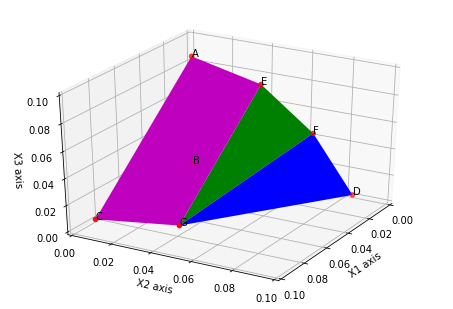
\includegraphics[width=0.5\textwidth]{pic1}
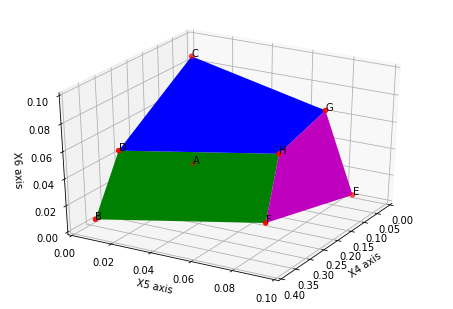
\includegraphics[width=0.5\textwidth]{pic2}

Грани, нарисованные синим, зелёным, фиолетовым цветом соответствуют первому, второму и третьему
неравенству каждой системы. Теперь проделаем алгоритм Лемке-Хоусона для одной из вершин.

\begin{center}
	\begin{tabular}{|c|c|c|c|c|}
		\hline
		$P_1$ & $P_2$ & метки $P_1$ & метки $P_2$ & удаляемая метка \\
		\hline
		B & A & 1 2 3 & 4 5 6 & 2\\
		\hline
		D & A & 1 3 4 & 4 5 6 & 4\\
		\hline
		D & B & 1 3 4 & 1 5 6 & 1\\
		\hline
		G & B & 3 4 5 6 & 1 5 6 & 6\\
		\hline
		G & D & 3 4 5 6 & 1 2 5 & $\times$\\
		\hline
	\end{tabular}
\end{center}

Таким образом, точка $(G, D) \sim (\frac{2}{3}, \frac{1}{3}, 0 \mid \frac{1}{7}, 0, \frac{6}{7})$
есть одно из смешанных равновесий.

\section*{Задача 4}

Убедимся, что эти задачи лежат в \textbf{TFNP}. Пусть $v$~--- вершина из первой задачи со степенью
$\deg(v)$, не делящейся на $p$. Если сумма степеней вершин в левой доле делится на $p$, то в левой
доле существует другая вершина $q$, такая что $\deg(q)$ не делится на $p$ (иначе вся сумма была бы
сравнима с $\deg(v)$). Если же сумма не сравнима с нулём, то аналогичным рассуждением заключаем, что
такая вершина существует справа.

Для задачи с ориентированным графом сумма балансов равна 0, поэтому по модулю $p$ существование
одной ненулевой вершины гарантирует существование другой.

Покажем, что они сводятся друг к другу. Сведем задачу в ориентированном графе к задаче в двудольном.
Для этого раздвоим вершины, сформировав две доли. Нам нужно добиться, чтобы степени вершин слева
совпадали с балансом вершин в исходном графе. Для этого мы можем провести ребро между $i$-й вершиной
левой доли и $j$-й вершиной правой доли если $(i, j)$ есть ребро в орграфе. Теперь степень $i$-й ш
вершины слева равна $outdeg(i)$, а справа $indeg(i)$. Тогда, если мы проведем $p - indeg(v) \bmod p$
между $i$ вершиной слева и справа, то слева степени вершины станут сравнивыми по модулю $p$ с
балансами, а справа сравнивыми с 0. Легко видеть, что все сведение является полиномиальным
преобразованием: по имеющейся полиномиальной функции $f$, перечисляющей входящие и исходящие вершины
в орграфе, строится соответствующая полиномиальная функция для двудольного графа.

Преобразование в обратную сторону проще: просто ориентируем рёбра слева направо. Тогда балансы
вершин слева такие же, как были степени, а балансы вершин справа стали минус степенями. Поскольку
минус на сравнимость с нулём не влияет, то все хорошо.

\section*{Задача 5}

\begin{center}
	\begin{tikzpicture}[->,>=stealth',shorten >=1pt,auto,node distance=2cm,semithick]
		\tikzstyle{every state}=[draw=black,text=white]

		\node[state] (X11) {};
		\node[state] (X12) [right of=X11] {};
		\node[state] (X13) [right of=X12] {};
		\node[state] (X21) [below of=X11] {};
		\node[state] (X22) [right of=X21] {};
		\node[state] (X23) [right of=X22] {};
		\node[state] (X31) [below of=X21] {};
		\node[state] (X32) [right of=X31] {};
		\node[state] (X33) [right of=X32] {};

		\path (X11) edge node {$x$} (X12);
		\path (X12) edge node {$x$} (X13);
		\path (X21) edge node {$2x$} (X22);
		\path (X22) edge node {$2x$} (X23);
		\path (X31) edge node {$x$} (X32);
		\path (X32) edge node {$x$} (X33);

		\path (X11) edge node {$x$} (X21);
		\path (X21) edge node {$x$} (X31);
		\path (X12) edge node {$2x$} (X22);
		\path (X22) edge node {$2x$} (X32);
		\path (X13) edge node {$x$} (X23);
		\path (X23) edge node {$x$} (X33);
	\end{tikzpicture}
	\hspace*{1cm}
	\begin{tikzpicture}[->,>=stealth',shorten >=1pt,auto,node distance=2cm,semithick]
		\tikzstyle{every state}=[draw=black,text=white]

		\node[state] (X11) {};
		\node[state] (X12) [right of=X11] {};
		\node[state] (X21) [below of=X11] {};
		\node[state] (X22) [right of=X21] {};
		\node[state] (X23) [right of=X22] {};
		\node[state] (X32) [right of=X31] {};
		\node[state] (X33) [right of=X32] {};

		\path (X11) edge node {$x$} (X12);
		\path (X21) edge node {$2x$} (X22);
		\path (X22) edge node {$2x$} (X23);
		\path (X32) edge node {$x$} (X33);

		\path (X11) edge node {$x$} (X21);
		\path (X12) edge node {$2x$} (X22);
		\path (X22) edge node {$2x$} (X32);
		\path (X23) edge node {$x$} (X33);

		\path (X12) edge node {$2x$} (X23);
		\path (X21) edge node {$2x$} (X32);
	\end{tikzpicture}
\end{center}

Понятно, что схемы выше эквивалентны. В силу симметрии по рёбрам из истока будет проходить
одинаковое количество потока равное $\frac{1}{2}$. Чтобы все пути имели одинаковый вес, нужно, чтобы
поток на развилке делился в отношении $1:2$, поэтому по центральных рёбрам будет течь $\frac{1}{6}$,
а по побочным $\frac{1}{3}$. Стоимость этого потока равна $4 \cdot \frac{1}{4} +
4 \cdot \frac{2}{36} + 2 \cdot \frac{2}{9} = 1 + \frac{6}{9} = \frac{5}{3}$. Найдём теперь
оптимальный поток: он равен равновесному потоку в сети, где все стоимости рёбер умножены на 2 (так
как $(cx \cdot x)' = 2cx$), то есть равновесный поток совпадает с оптимальным.

\section*{Задача 7}

Пусть природа играет так: на $i$-м ходу нужно сыграть стратегию $i \bmod 3 + 1$, чтобы получить
потери $0$, все остальные ходы дают потери $1$. Тогда если игрок <<перепутал>> стратегии 1 и 2, то
он получает потери $\frac{2T}{3}$. Сожаление второго рода при этом равно $\frac{2T}{3}$, так как
одна транспозиция даёт верную стратегию. Но сожаление первого рода равно 0 (стационарная стратегия
имеет такие же потери), поэтому нам надо немного <<ухудшить>> его стратегию, чтобы сожаление
первого рода стало положительным, но небольшим. Для этого просто каких-то моментах, когда игрок
правильно угадывает (это происходит на ходах вида $3k + 1$), изменим его стратегию. Пусть мы
изменили его решение в $k = k(T)$ моментах. От этого сожаление второго рода уменьшится на $O(k)$, а
сожаление первого рода станет ровно $k$.  Тогда выбрав, например, $k = \sqrt{T}$, получим
отношение, равное $\frac{\frac{2T}{3} - O(k)}{k} \sim \frac{2}{3}\sqrt{T} \rightarrow \infty$.

\section*{Задача 9}

Будем искать симметричное равновесие в классе абсолютно непрерывных распределений. Также попробуем
найти распределение с носителем плотности $\supp f(x) \supset (0; 1)$ и функцией распределения
$F(x) = \int_0^x f(x) dx$.

Так как смешиваются все <<чистые>> стратегии, то они должны приносить одинаковый ожидаемый доход.
Доход от чистой стратегии сыграть $x$, если все остальные играют распределение $F$ равен
$F(x)^{n-1} \cdot 1 - x = const$. Однако, эта константа равна 0, так как доход стратегии сыграть 0
равен 0. Стало быть $F(x) = x^\frac{1}{n-1}$.

Рассмотрим теперь какое-то другое распределение $G(x)$ c плотностью $g(x)$ (не обязательно с
носителем, содержащим $(0;1)$). Ожидаемый выигрыш этого распределения равен:

$$ \int_0^1 F(x)^{n-1} g(x) dx - \int_0^1 x g(x) = \int_0^1 xg(x) - \int_0^1 x g(x) = 0. $$

Рассуждение можно обобщить: если мы отклоняемся в распределение, не являющееся абсолютно
непрерывным, мы можем приблизить его случайной величиной с конечным числом значений, как в
определении матожидания. Для них верно аналогичное равенство, значит в пределе матожидание выигрыша
при отклонении все равно равно 0.

\section*{Задача 10}

а) Пусть оценки упорядочились как $V_{(1)} > \ldots > V_{(n)}$. Тогда в механизме VCG одноместная
комната достается обладателю наибольшей оценки, следующие двое по величине занимают двухместную
комнату. Назовём этих игроков условно <<первый>>, <<второй>> и <<третий>>. Также будем считать, что
есть <<четвёртый>> игрок, если его нет, то добавим фиктивного человека с оценкой 0.

Посчитаем платёж первого: он равен полезности, если бы первого игрока вообще не было минус
полезность, если бы не было его и одноместной комнаты:
$$ V_{(2)} + \frac{2}{3}(V_{(3)} + V_{(4)}) - \frac{2}{3}(V_{(2)} + V_{(3)}) = \frac{1}{3} V_{(2)} +
\frac{2}{3} V_{(4)}. $$
Платежи второго и третьего рассчитываются по тому же принципу:
$$ V_{(1)} + \frac{2}{3}(V_{(i)} + V_{(4)}) - V_{(1)} - \frac{2}{3}V_{(i)} = \frac{2}{3}V_{(4)}. $$

Ожидаемый доход тогда равен $EX = EV_{(2)} + 3\frac{2}{3}EV_{(4)}$. Из статистики знаем, что
плотность $V_{(k)}$ равна:
$$ f_{V_{(k)}} = \frac{n!}{(k-1)!(n-k)!} F^{n-k}(x) (1 - F(x))^{k-1} f(x) =
\frac{n! \cdot x^{n-k} (1-x)^{k-1}}{(k-1)!(n-k)!}. $$
Для равномерных величин это бета-распределение с матожиданием $\frac{n-k+1}{n+1}$. Поэтому доход от
механизма равен (в случае, если $n \ge 4$):
$$ R = \frac{n-1}{n+1} + 2\cdot \frac{n-3}{n+1} = \frac{3n-7}{n+1}. $$
Видим, что случай $n = 3$ в эту формулу вписывается.

б) Заметим снова, что комнаты будут расрпделены между людьми с тремя наибольшими оценками (если их
оценка больше, чем $C$). Докажем, что мы отдадим одноместную комнату человеку с максимальной
оценкой. Если $V_{(1)} < C$, то никто никуда не селится. Если $V_{(1)} > V_{(2)} > 1.5C$, то
полезность равна старой минус $2C$, поэтому выгодно все оставить так. Если же теперь $V_{(1)} > C$,
но $C < V_{(2)} < 1.5C$, то общая полезность равна либо $V_{(1)} - C$, либо $V_{(2)} + \frac{2}{3}
V_{(1)} - 2C \le \frac{2}{3}V_{(2)} + V_{(1)} - 2C \le V_{(1)} - C$. Второе меньше.

Далее, нужно сложить следующие случаи:
\begin{itemize}
	\item $V_{(1)} < C$, $R = 0$. Далее везде $V_{(1)} > C$
	\item $V_{(2)} < C$. Платёж первого тогда 0, остальные не селятся, а доход $R = -C$
	\item $C < V_{(2)} < 1.5C$. Платёж первого теперь $V_{(2)} - C$, остальные не селятся, $R =
		V_{(2)} - 2C$
	\item $V_{(2)} > 1.5C$, но $V_{(3)} < 1.5C$. Селятся первые двое, первый платит $V_{(2)} - C -
		\frac{2}{3}V_{(2)} + C = \frac{1}{3} V_{(2)}$, второй платит 0. Доход получается $\frac{1}{3}
		V_{(2)} - 2C$
	\item $V_{(3)} > 1.5C$, но $V_{(4)} < 1.5C$. Селятся первые трое, первый платит
		$\frac{1}{3} V_{(2)}$, второй и третий платят 0. Доход получается $\frac{1}{3}V_{(2)} - 3C$
	\item $V_{(4)} > 1.5C$. Тогда платежи будут как в пункте а), доход $R = \frac{1}{3}V_{(2)} +
		2V_{(4)} - 3C$
\end{itemize}

\section*{Задача 12}

\begin{center}
	\begin{tikzpicture}[->,>=stealth',shorten >=1pt,auto,node distance=2cm,semithick]
		\tikzstyle{every state}=[draw=black,text=black]

		\node[state] (S0) {$S_0$};
		\node[state] (S1) [right=2cm of S0] {$S_1$};
		\node[state] (S2) [below=2cm of S1] {$S_2$};
		\node[state] (S3) [left=2cm of S2] {$S_3$};
		\node[state] (S4) [above left=1cm and 2cm of S3] {$S_4$};

		\path (S0) edge node {D} (S1);
		\path (S1) edge node {D} (S2);
		\path (S2) edge node {D} (S3);
		\path (S3) edge [bend right] node {D} (S4);
		\path (S4) edge node {D} (S0);

		\path (S0) edge [loop above] node {C} (S0);
		\path (S1) edge [bend left] node {C} (S0);
		\path (S2) edge node {C} (S0);
		\path (S3) edge node {C} (S0);
		\path (S4) edge [bend right] node {C} (S3);
	\end{tikzpicture}
\end{center}

Течение игры для автоматов $(M, M)$:
\begin{center}
	\begin{tabular}{|c|c|c|c|c|}
		\hline
		состояние $M_1$ & вывод $M_1$ & вывод $M_2$ & состояние $M_2$ & выигрыши\\
		\hline
		$S_0$ & D & D & $S_0$ & (1, 1)\\
		\hline
		$S_1$ & D & D & $S_1$ & (1, 1)\\
		\hline
		$S_2$ & D & D & $S_2$ & (1, 1)\\
		\hline
		$S_3$ & D & D & $S_3$ & (1, 1)\\
		\hline
		$S_4$ & C & C & $S_4$ & (2, 2)\\
		\hline
		$S_3$ & D & D & $S_3$ & (1, 1)\\
		\hline
		\ldots & \ldots & \ldots & \ldots & \ldots\\
		\hline
	\end{tabular}
\end{center}

Если первый игрок однократно отклонится в какой-то момент и сыграет $C$ вместо $D$, то ход игры
будет следующим:

\begin{center}
	\begin{tabular}{|c|c|c|c|c|c|}
		\hline
		состояние $M_1$ & вывод $M_1$ & вывод $M_2$ & состояние $M_2$ & выигрыши & изменение $M_1$ \\
		\hline
		$S_i$ & C & D & $S_i$ & (0, 3) & $-1$\\
		\hline
		$S_{i+1}$ & D & D & $S_0$ & (1, 1) & $0$\\
		\hline
		\ldots & \ldots & \ldots & \ldots & \ldots & \ldots \\
		\hline
		$S_{4}$ & C & D & $S_{3-i} $ & (0, 3) & $-\delta^{4-i}$\\
		\hline
		$S_{0}$ & D & D & $S_{0} $ & (1, 1) & $0$\\
		\hline
		\ldots & \ldots & \ldots & \ldots & \ldots & \ldots \\
		\hline
	\end{tabular}
\end{center}

Видно что тут и далее на несколько нерасписанных шагов все изменения отрицательны. Остался вариант
отклонения в $D$, когда нам говорят $C$. Тогда ход игры будет таким:
\begin{center}
	\begin{tabular}{|c|c|c|c|c|c|}
		\hline
		состояние $M_1$ & вывод $M_1$ & вывод $M_2$ & состояние $M_2$ & выигрыши & изменение $M_1$ \\
		\hline
		$S_4$ & D & C & $S_4$ & (3, 0) & $+1$\\
		\hline
		$S_3$ & D & D & $S_0$ & (1, 1) & $0$\\
		\hline
		$S_4$ & C & D & $S_1$ & (0, 3) & $-2\delta^2$\\
		\hline
		$S_0$ & D & D & $S_0$ & (1, 1) & $0$\\
		\hline
		$S_1$ & D & D & $S_1$ & (1, 1) & $-\delta^4$\\
		\hline
		$S_2$ & D & C & $S_2$ & (1, 1) & $0$\\
		\hline
		$S_3$ & D & C & $S_3$ & (1, 1) & $-\delta^6$\\
		\hline
		$S_4$ & C & C & $S_4$ & (2, 2) & $+\delta^7$\\
		\hline
		$S_3$ & D & D & $S_3$ & (1, 1) & $-\delta^8$\\
		\hline
		$S_4$ & C & C & $S_4$ & (2, 2) & $+\delta^9$\\
		\hline
		\ldots & \ldots & \ldots & \ldots & \ldots & \ldots \\
		\hline
	\end{tabular}
\end{center}

То есть нас интересует, когда $1 - 2\delta^2 - \delta^4 - \delta^6(1 - \delta + \delta^2 + \ldots) =
1 - 2\delta^2 - \delta^4 - \delta^6 \frac{1}{1 + \delta} < 0$. Единственный положительный корень
этого уравнения равен $\approx 0.63266$, то есть $\delta \ge \approx 0.63266$.

Рассмотрим теперь игру $M'$ vs $M'$:
\begin{center}
	\begin{tabular}{|c|c|c|c|c|}
		\hline
		состояние $M'_1$ & вывод $M'_1$ & вывод $M'_2$ & состояние $M'_2$ & выигрыши \\
		\hline
		$S_0$ & D & D & $S_0$ & (1, 1) \\
		\hline
		$S_1$ & D & D & $S_1$ & (1, 1) \\
		\hline
		$S_2$ & D & D & $S_2$ & (1, 1) \\
		\hline
		$S_4$ & C & C & $S_4$ & (2, 2) \\
		\hline
		$S_3$ & D & D & $S_3$ & (1, 1) \\
		\hline
		$S_4$ & C & C & $S_4$ & (2, 2) \\
		\hline
		\ldots & \ldots & \ldots & \ldots & \ldots \\
		\hline
	\end{tabular}
\end{center}

А теперь допустим первый игрок решил поменять свой автомат на $M$:
\begin{center}
	\begin{tabular}{|c|c|c|c|c|c|}
		\hline
		состояние $M_1$ & вывод $M_1$ & вывод $M'_2$ & состояние $M'_2$ & выигрыши & изменение \\
		\hline
		$S_0$ & D & D & $S_0$ & (1, 1) & $0$\\
		\hline
		$S_1$ & D & D & $S_1$ & (1, 1) & $0$\\
		\hline
		$S_2$ & D & D & $S_2$ & (1, 1) & $0$\\
		\hline
		$S_3$ & D & C & $S_4$ & (3, 0) & $+\delta^3$\\
		\hline
		$S_0$ & D & D & $S_0$ & (1, 1) & $0$ \\
		\hline
		$S_1$ & D & D & $S_1$ & (1, 1) & $-\delta^5$\\
		\hline
		$S_2$ & D & D & $S_2$ & (1, 1) & $0$\\
		\hline
		$S_3$ & D & C & $S_4$ & (3, 0) & $+\delta^7$\\
		\hline
		$S_0$ & D & D & $S_0$ & (1, 1) & $0$\\
		\hline
		\ldots & \ldots & \ldots & \ldots & \ldots \\
		\hline
	\end{tabular}
\end{center}

Видно, что изменение такой стратегии образуют знакопеременную убывающую геометрическую прогрессию,
сумма у неё, конечно, положительна, поэтому первый отклонится.

\end{document}
